\documentclass{article}
\usepackage{amsmath, amssymb, tikz, tkz-euclide, tcolorbox, array, sfmath, enumerate, pgfplots, multicol}
\renewcommand{\familydefault}{\sfdefault}
\pgfplotsset{compat=newest}
\usetikzlibrary{arrows.meta}
\everymath{\displaystyle}
\tikzset{>=stealth}
\tikzstyle{input} = [circle, text centered, radius = 1cm, draw = black]
\tikzstyle{function} = [rectangle, text centered, minimum width = 2cm, minimum height = 1cm, draw = black]
\usepackage[top = 0.25in, bottom = 0.25in, left = 1in, right = 1in]{geometry}
\pagestyle{empty}
\raggedright

\newcounter{example}[section]
\newenvironment{example}[1][]{\refstepcounter{example}\par\medskip
   {\color{red}\textbf{Example~\theexample. #1}}}{\medskip}

\begin{document}

\section*{Compound Inequalities}

\begin{tcolorbox}[colframe=orange!70!white, coltitle=black, title=\textbf{Summary}]
\begin{enumerate}
    \item Compound inequalities means solving more than one inequality.
    \item The word \textit{and} indicates a number must make \underline{both} inequalities true.
    \item The word \textit{or} indicates a number must make \underline{at least one} inequality true.
\end{enumerate}
\end{tcolorbox}
\bigskip 

\subsection*{Compound Inequalities -- AND}

Compound inequalities involve inequalities connected by either the word {\color{blue}\textbf{and}} or the word {\color{red}\textbf{or}}.	
\bigskip 

A number is a solution to a compound inequality that involves the word \emph{and} if it is a solution to \textbf{\underline{both}} inequalities.

\[x \geq -1 \textbf{ and } x < 2\]

\begin{center}
	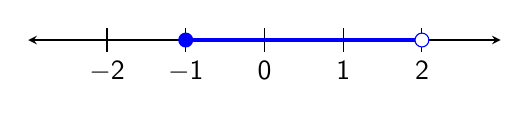
\begin{tikzpicture}
		\draw[<->](-3,0)--(3,0);
		\foreach \x in {-2,-1,...,2}
		\draw(\x,0.15)--(\x,-0.15) node [below] {$\x$};
		\draw[color=blue,fill=blue] (-1,0) circle [radius = 2.5pt];
		\draw[color=blue, ultra thick] (-1,0)--(2,0);
		\draw[color=blue, fill=white] (2,0) circle [radius=2.5pt];
	\end{tikzpicture}	
\end{center}

If you graph each individual inequality, the solution is the part of the number where they {\color{blue}\textbf{overlap}}.
\bigskip 

\begin{example}
Solve each. Graph your answers on a number line.
\begin{enumerate}[(a)]
\begin{multicols}{2}
    \item $2x-7<3 \quad \text{and} \quad 5x-4\geq 6$  
    \item $2x + 7 < 27 \quad \text{and} \quad 5x + 5 < -30$
\end{multicols}
\end{enumerate}
\end{example}

\vfill 

Sometimes, your variable is between two values, like in
\[
-3 < x < 7
\]

This really means 2 things:
\begin{enumerate}
    \item $x > -3$ AND
    \item $x < 7$
\end{enumerate}

So split it up into 2 inequalities and solve.

\vspace{0.5in}
\newpage 

\begin{example} 
Solve and graph each.	
\begin{enumerate}[(a)]
\begin{multicols}{2}
    \item $-3 < 2x + 1 \leq 3$
    \item $1 \leq 2x + 3 < 11$
\end{multicols}
\end{enumerate}
\end{example}

\vfill 

\subsection*{Compound Inequalities -- OR}
	The word \textbf{or} indicates the solution be in {\color{blue}\textbf{either}} inequality (or both).	\newline\\
	\[x > 2 \text{ or } x \leq -1\]
	\begin{center}
		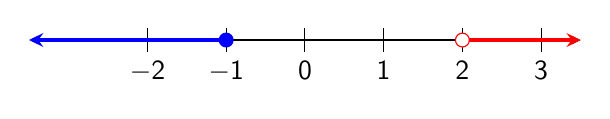
\begin{tikzpicture}
			\draw[<->] (-3.5,0) -- (3.5,0);
			\foreach \x in {-2,-1,...,3}
			\draw (\x,0.15) -- (\x,-0.15) node [below] {$\x$};
			\draw[->,blue,very thick] (-1,0) -- (-3.5,0);
			\draw[color=blue,fill=blue] (-1,0) circle [radius=2.5pt];
			\draw[->,red,very thick] (2,0) -- (3.5,0);
			\draw[color=red,fill=white] (2,0) circle [radius=2.5pt];
		\end{tikzpicture}
	\end{center}
\bigskip 

With the word \texttt{OR}, you can graph both on the number line at the same time.
\bigskip 

\begin{example}
Solve and graph each.
\begin{enumerate}[(a)]
    \item $2x-3<7 \quad \text{or} \quad 35-4x \leq 3$        \vfill 
    \item $x + 10 < 13 \quad \text{or} \quad 22 > x + 10$       \vfill 
    \item $4x + 2 > -22 \quad \text{or} \quad 26 \geq 4x + 2$   \vfill 
\end{enumerate}
\end{example}

\end{document}
